% Figures for main.tex.
%
% EVERY coordinate below is read verbatim out of a committed artifact under docs/benchmarks/, and
% scripts/check-paper-numbers.py fails if any number here is absent from one. No value is derived,
% interpolated, or nudged to make a curve look better — if a shape looks wrong, regenerate the
% artifact; do not move the point.
%
% Sources:
%   Fig. 2 cost-quality plane   docs/benchmarks/mbpp-974-opus.txt      (RouterBench metric block)
%   Fig. 3 threshold sweep      docs/benchmarks/mbpp-974-sonnet-k5.txt (imperfect-gate sweep)

% Palette — chosen for white paper stock and checked to stay distinguishable in greyscale, since
% reviewers still print. Hue carries meaning consistently across all three figures:
%   teal = Firstpass / the verified path   amber = the gate and its threshold
%   red  = failure, wrong answers served    slate = baselines and prior art
\definecolor{fpteal}{HTML}{0E8F73}
\definecolor{fpamber}{HTML}{B5730B}
\definecolor{fpred}{HTML}{C0392B}
\definecolor{fpslate}{HTML}{51606F}
\definecolor{fpmist}{HTML}{DDE4EA}

% ---------------------------------------------------------------------------------------------
% Fig 1 — architecture: what happens per request, and what it leaves behind.
% ---------------------------------------------------------------------------------------------
\begin{figure}[t]
\centering
\begin{tikzpicture}[
  font=\small,
  box/.style={draw=fpslate, fill=fpmist!45, rounded corners=3pt, minimum height=9.5mm,
              align=center, inner xsep=3.5mm, thick},
  cheap/.style={box, draw=fpteal, fill=fpteal!10},
  toprung/.style={box, draw=fpslate, fill=fpslate!12},
  gate/.style={draw=fpamber, fill=fpamber!12, rounded corners=3pt, minimum height=11mm,
               align=center, inner xsep=4mm, very thick},
  served/.style={box, draw=fpteal, fill=fpteal!22},
  rec/.style={draw=fpslate, dashed, fill=white, rounded corners=3pt, align=center,
              inner xsep=3mm, thick},
  arr/.style={-{Latex[length=2.2mm]}, semithick, fpslate},
  lbl/.style={font=\scriptsize, text=fpslate},
]
\node[box] (req) {request};
\node[cheap, right=7mm of req] (m0) {rung $m_1$\\[-1pt]\scriptsize cheapest};
\node[gate, right=7mm of m0] (g) {gate $g(y)$\\[-1pt]\scriptsize reads the \emph{output}};
\node[served, right=8mm of g] (serve) {serve};
\node[toprung, below=8mm of g] (m1) {rung $m_2$\\[-1pt]\scriptsize next rung};
\node[rec, below=8mm of m0] (r) {hash-chained receipt\\[-1pt]\scriptsize rung · verdict · score · cost · $h_{i-1}$};

\draw[arr] (req) -- (m0);
\draw[arr] (m0) -- node[lbl, above] {$y_1$} (g);
\draw[arr, draw=fpteal] (g) -- node[lbl, above, text=fpteal] {$g(y)\!\ge\!\tau$} (serve);
\draw[arr, draw=fpred] (g) -- node[lbl, right, text=fpred, xshift=0.5mm] {fail} (m1);
\draw[arr] (m1) -| ($(m0.south east)+(3mm,0)$) |- ($(g.west)+(0,-3mm)$);
\draw[arr, dashed] (g) -- (r);
\end{tikzpicture}
\caption{Verified cascade routing. The gate reads the \emph{output}, so the decision is made once
the evidence that settles it exists --- unlike prompt-conditioned routing, which must commit
before that evidence exists. Escalation is one rung and budget-capped. Every attempt, including
rejected ones, is billed and written to a hash-chained receipt an auditor can re-derive from
stored records alone.}
\label{fig:arch}
\end{figure}

% ---------------------------------------------------------------------------------------------
% Fig 2 — cost-quality plane against RouterBench's Zero Router.
% ---------------------------------------------------------------------------------------------
\begin{figure}[t]
\centering
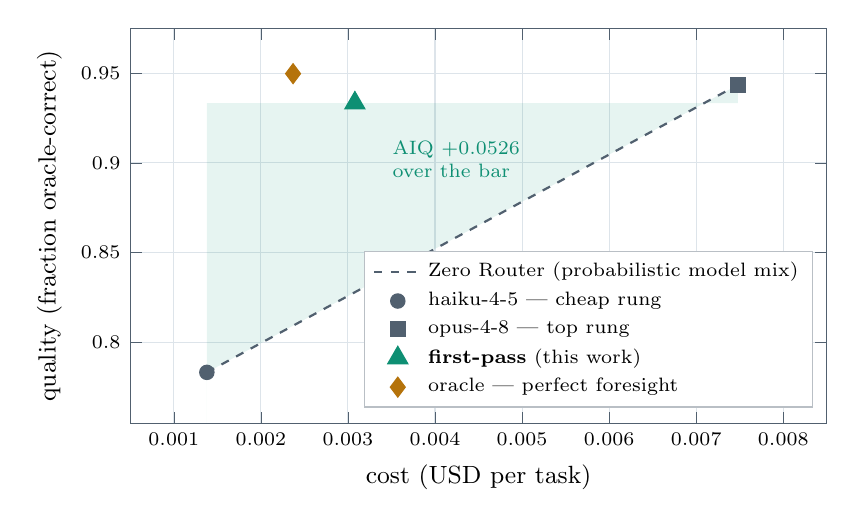
\begin{tikzpicture}
\begin{axis}[
  width=0.86\linewidth, height=6.6cm,
  xlabel={cost (USD per task)}, ylabel={quality (fraction oracle-correct)},
  xmin=0.0005, xmax=0.0085, ymin=0.755, ymax=0.975,
  scaled x ticks=false,
  xticklabel style={/pgf/number format/fixed, /pgf/number format/precision=4, font=\scriptsize},
  yticklabel style={font=\scriptsize},
  label style={font=\small}, axis line style={fpslate}, tick style={fpslate},
  grid=major, grid style={fpmist},
  legend style={font=\scriptsize, draw=fpslate!40, fill=white,
                at={(0.98,0.04)}, anchor=south east},
  legend cell align=left,
]
% Band between the two measured model points and first-pass's measured quality. Every vertex is
% a measured value; nothing here is interpolated.
\addplot[draw=none, fill=fpteal, fill opacity=0.10, forget plot]
  coordinates {(0.00138,0.7834) (0.00748,0.9435) (0.00748,0.9333) (0.00138,0.9333)} \closedcycle;

\addplot[thick, fpslate, dashed] coordinates {(0.00138,0.7834) (0.00748,0.9435)};
\addlegendentry{Zero Router (probabilistic model mix)}
\addplot[only marks, mark=*, mark size=2.6pt, fpslate] coordinates {(0.00138,0.7834)};
\addlegendentry{haiku-4-5 --- cheap rung}
\addplot[only marks, mark=square*, mark size=2.6pt, fpslate] coordinates {(0.00748,0.9435)};
\addlegendentry{opus-4-8 --- top rung}
\addplot[only marks, mark=triangle*, mark size=4.2pt, fpteal] coordinates {(0.00308,0.9333)};
\addlegendentry{\textbf{first-pass} (this work)}
\addplot[only marks, mark=diamond*, mark size=3.6pt, fpamber] coordinates {(0.00237,0.9497)};
\addlegendentry{oracle --- perfect foresight}

\node[font=\scriptsize, text=fpteal, anchor=west, align=left]
  at (axis cs:0.0034,0.902) {AIQ $+0.0526$\\over the bar};
\end{axis}
\end{tikzpicture}
\caption{Cost--quality plane, 974 MBPP tasks with real unit-test gates
(\texttt{mbpp-974-opus.txt}). The dashed line is RouterBench's \emph{Zero Router}: every point on
it is reachable by dispatching probabilistically between the two models, so it is the bar below
which a router has accomplished nothing at all. first-pass lies above it; the shaded band is the
region it opens up. Integrated across the cost domain this is an AIQ lift of $+0.0526$ --- 72\% of
the headroom to perfect foresight. RouterBench reports \emph{no} learned router significantly
clearing this bar, and routers scoring worse than it on MBPP specifically.}
\label{fig:plane}
\end{figure}

% ---------------------------------------------------------------------------------------------
% Fig 3 — the sweep. The production threshold is dominated, not merely conservative.
% ---------------------------------------------------------------------------------------------
\begin{figure}[t]
\centering
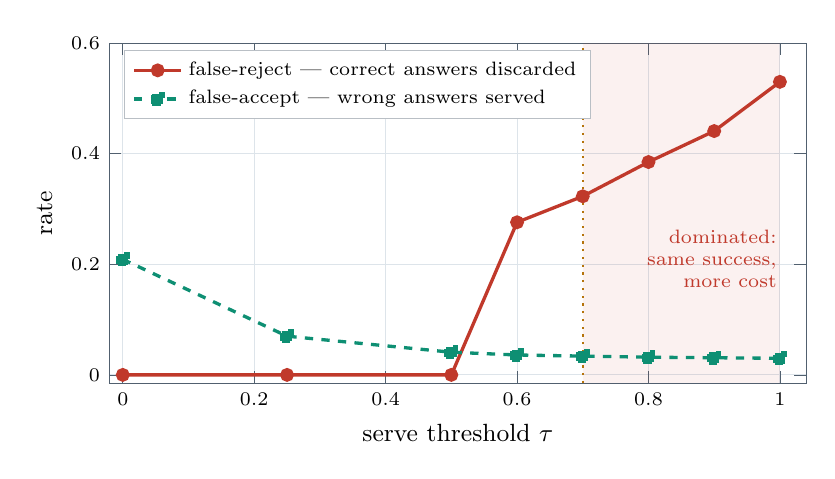
\begin{tikzpicture}
\begin{axis}[
  width=0.86\linewidth, height=5.9cm,
  xlabel={serve threshold $\tau$}, ylabel={rate},
  xmin=-0.02, xmax=1.04, ymin=-0.015, ymax=0.60,
  xticklabel style={font=\scriptsize}, yticklabel style={font=\scriptsize},
  label style={font=\small}, axis line style={fpslate}, tick style={fpslate},
  grid=major, grid style={fpmist},
  legend style={font=\scriptsize, draw=fpslate!40, fill=white,
                at={(0.02,0.98)}, anchor=north west},
  legend cell align=left,
]
% The band from tau=0.70 to tau=1.00: identical success, strictly higher cost.
\addplot[draw=none, fill=fpred, fill opacity=0.07, forget plot]
  coordinates {(0.70,-0.015) (1.00,-0.015) (1.00,0.60) (0.70,0.60)} \closedcycle;

\addplot[very thick, fpred, mark=*, mark size=1.9pt] coordinates {
  (0.00,0.000) (0.25,0.000) (0.50,0.000) (0.60,0.276) (0.70,0.323) (0.80,0.385)
  (0.90,0.441) (1.00,0.530)};
\addlegendentry{false-reject --- correct answers discarded}

\addplot[very thick, fpteal, dashed, mark=square*, mark size=1.9pt] coordinates {
  (0.00,0.209) (0.25,0.070) (0.50,0.041) (0.60,0.036) (0.70,0.034) (0.80,0.032)
  (0.90,0.031) (1.00,0.030)};
\addlegendentry{false-accept --- wrong answers served}

\draw[fpamber, thick, dotted] (axis cs:0.70,-0.015) -- (axis cs:0.70,0.60);
\node[font=\scriptsize, text=fpamber, anchor=south east] at (axis cs:0.69,0.45) {$\tau=0.70$};
\node[font=\scriptsize, text=fpred, anchor=north east, align=right]
  at (axis cs:1.01,0.28) {dominated:\\same success,\\more cost};
\end{axis}
\end{tikzpicture}
\caption{Gate error against the serve threshold, on the judged run --- the only configuration
measured with a \emph{graded} gate score, since the unit-test gate alone is binary on MBPP
(\texttt{mbpp-974-sonnet-k5.txt}). The production policy serves at $\tau=1.0$, where the gate
discards \textbf{53\%} of cheap answers that were in fact correct, paying for escalations that
were never needed. False-accept barely moves across the shaded band (0.030 at $\tau=1.0$ against
0.034 at $\tau=0.70$), so that strictness buys almost no safety. Success at $\tau=0.70$ is
\emph{identical} (0.9271) at 12\% lower cost per success: the production threshold is dominated,
not merely conservative.}
\label{fig:sweep}
\end{figure}
